%
% Chapter 1
%
% Unifies results chapters under the framework of human genetics.

% TODO: look through dloads folder for relevant papers for each section

\chapter{Introduction}
\label{ch:discussion}

\begin{outline}


\1 Observable human characteristics or traits are called phenotypes.
    \2 Variation in phenotype emerges from the interplay of genetics, environment and pure chance.
    \2 Traits for which genetic variation explains a non-zero fraction of phenotypic variation are heritable.
    \2 Virtually all phenotypic traits are heritable to some degree, and twin studies provide upper bounds on this heritability by partitioning phenotypic variation in to genetic and environmental components \url{https://www.nature.com/articles/ng.3285}.

\1 Genetic variation presents a unique opportunity to probe the causal molecular mechanisms underlying phenotypes.
    \2 Information encoded in the genome flows through multiple molecular layers (\autoref{fig:intro_sysBio}).
    % TODO: mechs not explicity mentioned, PTMs, epigenetic reg, Reverse transcription, RNA editing, predom flow of info holds.
    \2 A guiding principle is the central dogma, whereby the flow is unidirectional from DNA to RNA to protein via transcription and translation.
    \2 Barring somatic mutation, an individual's genome is fixed at conception, providing a causally upstream anchor.
    \2 Genetic association studies hence have intrinsic resistance to unmeasured confounding and reverse causality, issues that permeate observational studies of the causes of human phenotypes.
    % TODO: genetic markers are measured with relatively little error
    % TODO: https://twitter.com/GENES_PK/status/1283736619133149185
\1 A mainstay of the field of human genetics is discovering the specific genetic variants that contribute to heritability of each phenotype through statistical association of variants and phenotypes.

\begin{figure}
    \centering
    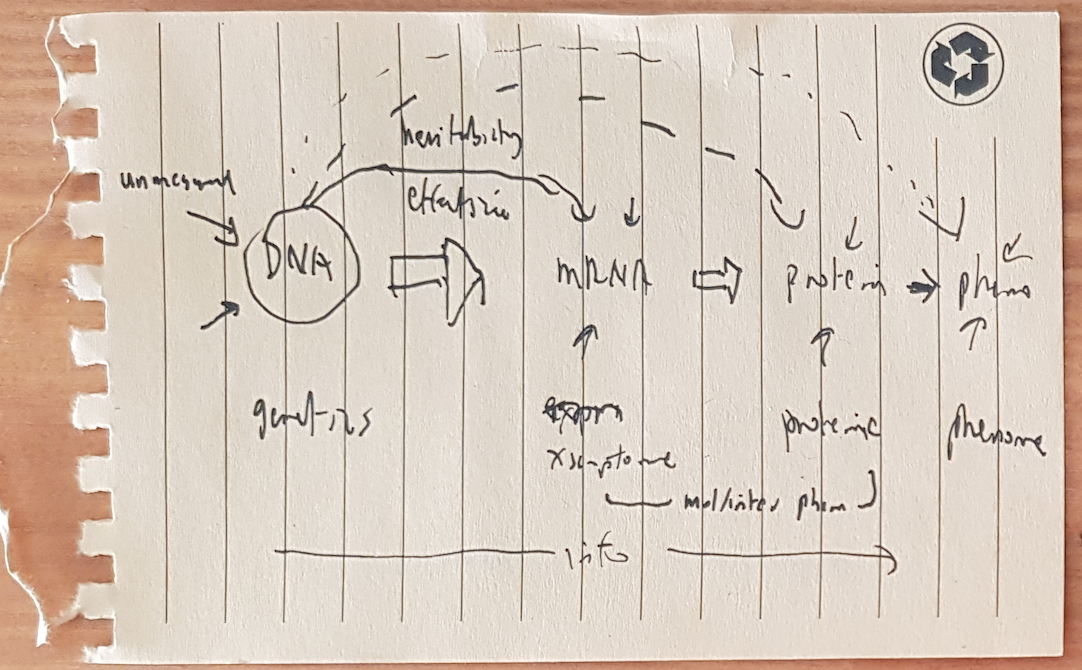
\includegraphics[width=1.0\textwidth,page=1]{mainmatter/figures/chapter_01/fig_mockup_systemsBio_Screenshot 2020-05-21 at 17.08.47.png}
    \caption{Information flow through the biological system.}
    \label{fig:intro_sysBio}
\end{figure}

\section{Genetic association studies of complex traits}

\subsection{Structure and variation of the genome}

\1 The human genome is almost three billion \glspl{bp} in length, 
containing 20000-25000 protein-coding genes \autocite{theencodeprojectconsortium2012IntegratedEncyclopediaDNA,1000genomesprojectconsortium2015GlobalReferenceHuman} that span 1-3\% of its length, 
% TODO: update to encode 3
with the remainder being non-coding.
% Some of the the remainder is likely dedicated to regulatory activities \autocite{theencodeprojectconsortium2012IntegratedEncyclopediaDNA}.
Each diploid cell contains two copies of the genome, organised into 46 chromosomes comprised of 23 maternal-parental pairs: 22 pairs of homologous autosomes and one pair of sex chromosomes.
%
\1 Variation in the genome between individuals in a population exists in the form of \glspl{SNP}, short indels, and structural variants
The vast majority ($> 99.9\%$) of common population variants ($\text{\gls{MAF}} > 1-5\%$) are \glspl{SNP} and short indels \autocite{1000genomesprojectconsortium2015GlobalReferenceHuman}.
% https://www.ncbi.nlm.nih.gov/dbvar/content/overview/
% Structural variation (SV) is generally defined as a region of DNA
% approximately 1 kb and larger in size and can include inversions and
% balanced translocations or genomic imbalances (insertions and deletions),
% commonly referred to as copy number variants (CNVs).
On average, a pair of genomes differs by one \gls{SNP} per 1000-2000 \gls{bp} \autocite{theinternationalsnpmapworkinggroup2001MapHumanGenome}.
Each version of a variant is called an allele; an individual has a maternal and parental allele at each variant.
\todo{consider moving awkward defs to margin notes, in the style of nature reviews}

% The Law of Dominance: An organism with alternate forms of a gene will express the form that is dominant.
% Law of Segregation: states that a diploid organism passes a randomly selected allele for a trait to its offspring, such that the offspring receives one allele from each parent.
% Law of independent assortment: states that genes do not influence each other with regard to the sorting of alleles into gametes; every possible combination of alleles for every gene is equally likely to occur.
\1 The many variants in a population are inherited in a smaller number of haplotypes: 
contiguous stretches of the genome passed through generations via meiotic segregation.
The fundamental sources of genetic diversity are mutation and meiotic recombination, generating new alleles and breaking apart haplotypes into shorter ones over evolutionary time.
\todo{LD decay just takes a really really long time, but there are evo forces at work too that maintain LD}
Variants at locations on a chromosome (loci) that are physically close are less likely to flank a recombination event, hence more likely to cosegregate on the same haplotype, referred to as genetic linkage.
Genetic linkage is one source of \gls{LD}: the non-random association of alleles at two loci, differing from expectation based on their frequencies and the law of independent assortment \autocite{slatkin2008LinkageDisequilibriumUnderstanding}.
\gls{LD} is often quantified within a population by $r^2$, the squared correlation coefficient between alleles \autocite{slatkin2008LinkageDisequilibriumUnderstanding}.

Recombination events are not distributed uniformly throughout the genome.
The genome is a mosaic of blocks delimited by recombination hotspots, 
characterised by strong \gls{LD} within blocks, and little \gls{LD} between blocks \autocite{wall2003HaplotypeBlocksLinkage,theinternationalhapmapconsortium2007SecondGenerationHuman} (\autoref{fig:intro_haplotypeBlocks}).
\todo{Heard it's good for the reader's attention span to have figures in intro. Unless it's ok to use figures from papers, I only want to spend the time making the min that are necessary though.}
\todo{can I just cite and use published figures?}
The structure of correlated haplotypes reflects a population's unique evolutionary history, and can be used to trace the demography of populations back through time \autocite{karczewski2020AnalyticTranslationalGenetics}.

\begin{figure}
    \centering
    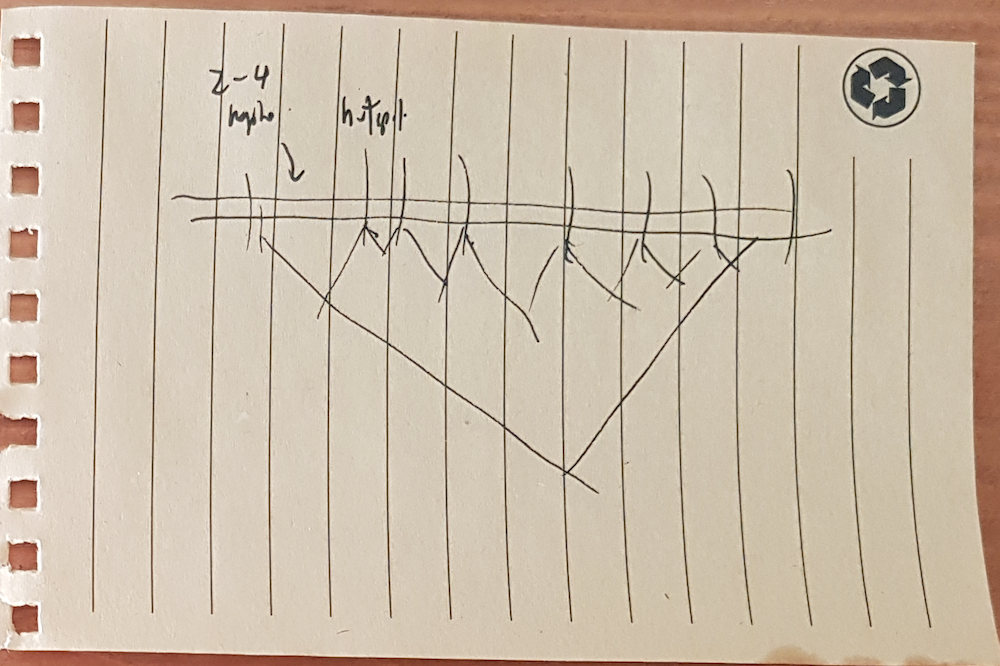
\includegraphics[width=1.0\textwidth,page=1]{mainmatter/figures/chapter_01/fig_mockup_haplotypeBlocks_Screenshot 2020-05-21 at 17.08.33.png}
    \caption{The genomic mosaic: block-like \gls{LD} structure of the genome}
    \label{fig:intro_haplotypeBlocks}
\end{figure}

\subsection{Lessons from the past 15 years}

\1 Genetic variants at loci in the genome can affect phenotype by impacting on the function or regulation of target genes.
How genetic variation contributes to a heritable trait defines it's genetic architecture: 
the number of genes affecting that trait; along with the allele frequencies, effect sizes, and interactions of trait-associated variants \autocite{visscher2019Fisher1918Paper}.
The number of genes defines a spectrum of traits from monogenic (where inheritance follows simple Mendelian patterns) to polygenic (where inheritance is complex).
Many architectures have been proposed for complex traits; all have in common that the number of genes that affect a complex trait is large (ranging from dozens to many thousands),
thus the average effect of each trait-associated locus is small \autocite{gibson2011RareCommonVariants,boyle2017ExpandedViewComplex} \url{https://www.pnas.org/content/106/23/9362}.

\1 For decades, linkage analysis had been successfully applied to map loci affecting Mendelian traits by tracing their cosegregation with traits through pedigrees \autocite{visscher2012FiveYearsGWAS}.
Small-scale genetic association studies were also performed, focusing on variants in or near candidate genes selected on the basis of prior biological knowledge \autocite{hirschhorn2002ComprehensiveReviewGenetic}.
These approaches were not successful for complex traits, as small effect sizes lead to low penetrance in pedigrees \autocite{visscher2012FiveYearsGWAS}
and poor power at the sample sizes typically used in early candidate gene studies \autocite{border2019NoSupportHistorical}.

\1 \Glspl{GWAS} systematically test common variants selected in a comparatively hypothesis-free manner across the genome for association with a trait (\autoref{fig:intro_architectureGWAS}).
Using large sample sizes to overcome small effects and large multiple testing burden, thousands of associations have been discovered for complex traits and disease,
many robustly replicated across populations \autocite{visscher2012FiveYearsGWAS,visscher201710YearsGWAS}.
Most genetic variance is explained by additive effects, the contribution of epistatic interactions is small \autocite{visscher2019Fisher1918Paper}, 
and genetic variants with effects on multiple phenotypes (pleiotropy) is widespread \autocite{visscher2012FiveYearsGWAS}.
Sample sizes in the millions are increasingly commonplace, 
% e.g. https://www.nature.com/articles/s41588-020-0637-y
and discovery of new associations with increasing sample size shows no sign of plateauing \autocite{tam2019BenefitsLimitationsGenomewide}.
    % TODO:
    % In general, effect size is inverse to frequency \url{https://twitter.com/Eric_Fauman/status/1301598386462887936?s=09}
    \2 These new associations have ever smaller effect sizes \url{https://www.pnas.org/content/early/2020/07/30/2005634117#F1}.
It is now appreciated that most heritable organism-level phenotypes are complex, and have remarkable polygenicity, with many hundreds or thousands of associated loci.
% TODO: any more takehomes from: \autocite{gallagher2018PostGWASEraAssociation,tam2019BenefitsLimitationsGenomewide}
% TODO recent omnigenic models liu et al 2019: every gene expressed in relevant tissues has non zero effect due to reg networks (mostly indirect through other genes)
    \2 In general, the more organism level a phenotype, the more polygenic, but even molecular traits are very polygenic
    % TODO: ref here is testosterone levels by pritchard
% TODO: also Polygenic background modifies penetrance of monogenic variants for tier 1 genomic conditions https://www.nature.com/articles/s41467-020-17374-3

% Genetic variants exist along a spectrum of allele frequencies and
% effect sizes. Most risk variants identified by GWAS lie within the two diagonal lines.
% Rare variants with small effect sizes are difficult to identify using GWAS, and common
% variants with large effects are unusual for common complex diseases.
% tam2019BenefitsLimitationsGenomewide
\begin{figure}
    \centering
    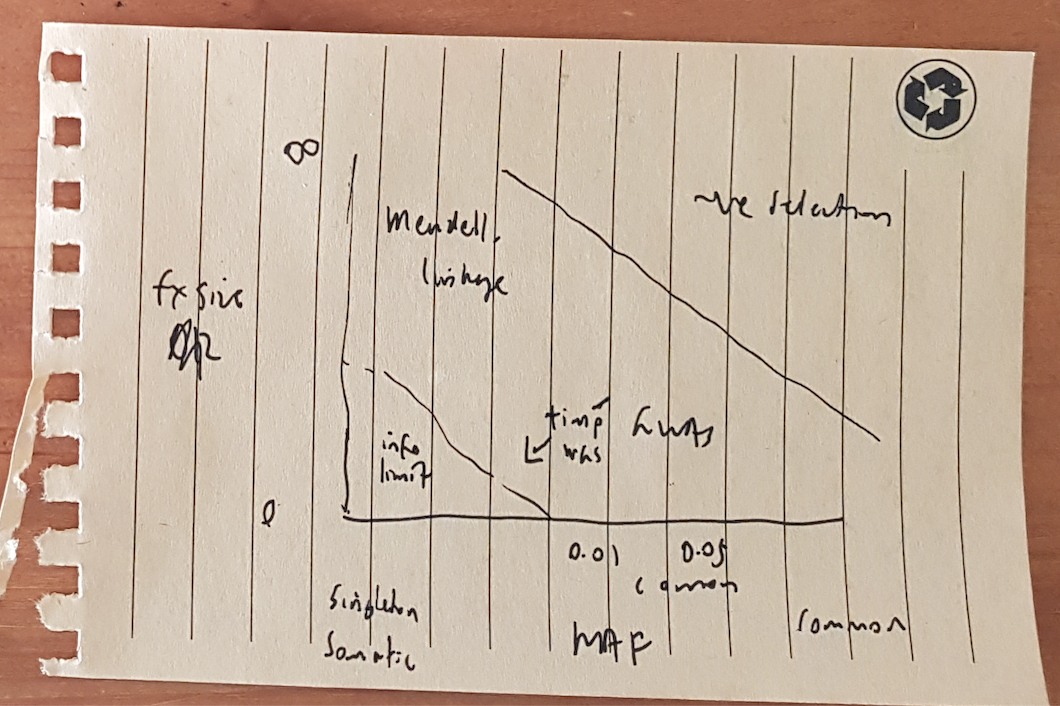
\includegraphics[width=1.0\textwidth,page=1]{mainmatter/figures/chapter_01/fig_mockup_architecture_Screenshot 2020-05-21 at 17.08.41.png}
    \caption{The reach of GWAS. OR vs MAF ala tam2019BenefitsLimitationsGenomewide, extended by imputation, sample size, WGS based genotypes, but may be indistinguishable from noise at the limits}
    \label{fig:intro_architectureGWAS}
\end{figure}

\subsection{From complex trait to locus}

\glspl{GWAS} rely on the tendency of common variants on the same haplotype to be in strong \gls{LD}.
As the number of haplotypes is comparatively few, 
it is possible to select a subset of tag variants such that all other known common variants are within a certain \gls{LD} threshold of that subset. 
In practice, there is enough redundancy that the number of variants measured on a modern genotyping array (in the order of \numrange[retain-unity-mantissa=false]{1e5}{1e6}) is sufficient to tag almost all common variants  \autocite{theinternationalhapmapconsortium2005HaplotypeMapHuman,barrett2006EvaluatingCoverageGenomewide}.
Associations with unmeasured variants are indirectly detected through their strong correlation with a tag variant.
Furthermore, as unrelated individuals still share short ancestral haplotypes, 
study samples can be assigned haplotypes from a panel of haplotypes derived from reference samples by matching on the directly genotyped variants.
This process of genotype imputation allows ascertainment of many more variants not directly genotyped \autocite{das2018GenotypeImputationLarge},
but helps to recover rarer variants that are poorly-tagged \autocite{visscher201710YearsGWAS}.
\todo{seems like there is some connection to be made between the tagability of common variation and the feasibility of imputation both being enabled by the relatively small number of common haplotypes compared to variants}
Modern imputation panels enable cost-effective \glspl{GWAS} including tens of millions of variants down to frequencies of \textapprox{0.01\%} \url{https://www.biorxiv.org/content/10.1101/563866v1}.

Testing such large numbers of variants incurs a massive multiple testing burden, but acknowledging the correlation between variants due to \gls{LD},
there are only the equivalent of \textapprox{10^6} independent tests in the European genome, regardless of the number of tests actually performed \autocite{peer2008EstimationMultipleTesting}.
The field has thus converged on a fixed discovery threshold of $0.05 / 10^6 = \num{5e-8}$ for genome-wide significance in European populations \autocite{jannot2015108HasEmerged}, akin\footnote{
    The Bonferroni procedure makes no assumptions about the dependence structure of the \pvalues{}, and is conservative (i.e. controls the \gls{FWER} at a stricter level than the chosen $\alpha$) even for independent tests. In fact it is always conservative unless the \pvalues{} have strong negative correlations \autocite{goeman2014MultipleHypothesisTesting}.
}
to controlling the family-wise type I error rate at using the Bonferroni correction.

% \todo{CUT: There is a limit, the strategy of association is fundamentally unsuited to rare variants.}
%
%     Rare Variants Association Analysis in Large-Scale Sequencing Studies at the Single Locus Level
%     https://doi.org/10.1371/journal.pcbi.1004993
%     Despite being extremely successful for common variants in GWA studies [43–46], procedures based on false-positive control are often underpowered in NGS studies involving rare variants (as illustrated in Fig 1).
%     In NGS studies with rare variants, the Signals region often degenerates due to extremely low MAF and high dimensionality.
%
% GWAS arrays don't tag rare variants very well:
%
% https://www.ncbi.nlm.nih.gov/pmc/articles/PMC3830981/
% When the allele frequencies of two loci are very different, the r2 will never
% be very large. To see this, let's assume pA<<PB and 1-pA≈1. Then the maximum
% r2≈pA/pB*(1-pB), which is <<1 since PA is very small compared to pB. This
% indicates that causal rare variants are mostly likely to be missed in GWAS for
% single marker tests, since GWAS chips are designed to include predominantly
% common variants (e.g. MAF>0.05).
%
% Therefore, GWASs are by design powered to detect association with causal variants that are relatively common in the population.
% \autocite{visscher2012FiveYearsGWAS}

% Also see:
% 2007: Wellcome Trust Case Control Consortium landmark GWAS
% 2009: Well-known paper: Finding the missing heritability of complex diseases https://www.ncbi.nlm.nih.gov/pmc/articles/PMC2831613/
% 2018: Revisiting the Missing Heritability of Complex Diseases, Ten Years On https://www.genome.gov/event-calendar/Revisiting-Missing-Heritability-of-Complex-Diseases-Ten-Years-On
%
% NOTE: a second approach to heritability estimation is linkage disequilibrium (LD) score regression.
%
% \todo{CUT: Missing heritability}
%
% \1 Missing heritability refers to the observation that SNP-based heritability estimates from \gls{GWAS} fall short of additive (narrow-sense) heritability estimates from traditional quantitative methods such as twin studies.
% Perhaps unsurprisingly, it has been hypothesised that the remaining heritability lies in variants that can not be assessed by \gls{GWAS} due to rarity or small effect.
% A classic example is the heritability of human height, estimated at 80\% by twin studies \autocite{maher2008PersonalGenomesCase},
% where considering only significant associations from \gls{GWAS} explains 5\% \autocite{maher2008PersonalGenomesCase}.
% Consideration of all common variants using mixed models (\software{GCTA}) increases the estimate to 45\% \autocite{yang2010CommonSNPsExplain},
% Recent work (\software{GREML-WGS}) suggests the full estimate of 80\% might be recoverable by also including rare and poorly tagged variants measured by \gls{WGS} \autocite{wainschtein2019RecoveryTraitHeritability}.

% \todo{CUT: WGS/WES migitates the coverage bias of GWAS towards known variation.}
%
% \1 approx 10-fold increase in variants per tech upgrade
% \1 WES/WGS is a trade-off between sample size and genomic coverage
%     \2 Allows tdiscovery and association with rare and novel variation, including structural variants.
%     \2 "In addition, other genome-wide scans, such as WES and WGS studies, allow testing for a burden of rare variants across shared functional units (e.g., genes) in a way that is not accessible to GWASs."
% \1 WES (covers about 40Mbp of the genome)
%     \2 covers more of the genome than GWAS
%     \2 but lower n, so lower power to do single variant associations
%     \2 needs 50x: variable coverage due to pulldown
% \1 WGS
%     \2 there is a tradeoff between variant capture (n needed to observe variant) and sequencing depth (gives confidence to call variants)
%     \2 20x ok to call 90\% of singletons
%     \2 rare variants, including in nc regions
%         \3 current discovery biases, finding higher effect size vars first
%         \3 burden tests (e.g. SAIGE)
%             \4 review \url{https://www.nature.com/articles/s41576-019-0177-4}
%     \2 also gets structural variants

\subsection{From locus to causal variant}

\1 By design, a significantly-associated variant from a \gls{GWAS} needs not be a variant that causally affects the trait, and may only tag a causal variant.
    \2 Fine-mapping is the process of determining which of the many correlated variants at a \gls{GWAS} locus are causal.
    % TODO: broekema2020PracticalViewFinemapping
    % For sparse enough problems, most other Bayesian methods provide posterior probabilities on "models" by enumerating (CAVIAR), schochastic search (FINEMAP) or sampling (BIMBAM) from all possible combinations of variables.
    % https://stephenslab.github.io/susie-paper/manuscript_results/motivating_example.html
    \2 State-of-the-art methods (e.g. PAINTOR, CAVIARBF, FINEMAP \url{https://www.ncbi.nlm.nih.gov/pmc/articles/PMC6050137/}, SuSiE) provide Bayesian posterior probabilities that associated variants are causal, and some methods can consider the presence of multiple causal variants at the same locus \autocite{schaid2018GenomewideAssociationsCandidate}.
    \2 Even if a single causal variant cannot be assigned, a credible set can be assigned.
    \2 Power: to separate causal and tag variants depends on \gls{LD} and sample size \autocite{visscher201710YearsGWAS}. \url{https://www.ncbi.nlm.nih.gov/pmc/articles/PMC6050137/}
    \2 Resolution: Naturally, these methods assign probabilities assuming the causal variant is in the set of variants observed.
        \3 The causal variant must either be genotyped or confidently imputed. Denser genotyping e.g. by WGS, and larger imputation panels will help.

% \subsection{Polygenic risk scores}
%
% Why care? PRS for prediction.
%
% First PRS
% 13. Wray, N.R., Goddard, M.E., and Visscher, P.M. (2007). Prediction of individual genetic risk to disease from genome-wide association studies. Genome Res. 17, 1520–1528.
%
% Variable prediction accuracy of polygenic scores within an ancestry group
% https://elifesciences.org/articles/48376
%
% Polygenic background modifies penetrance of monogenic variants conferring risk for coronary artery disease, breast cancer, or colorectal cancer
% https://www.medrxiv.org/content/10.1101/19013086v1

\subsection{From causal variant to target gene}

\1 Herein lies one of the greatest challenges of interpreting \gls{GWAS} results.
\1 For variants in coding regions (nonsense, missense, frameshift), there is a reasonable prior as to the target gene.
\1 Unlike for Mendelian traits where most causal variants are coding \url{https://www.ncbi.nlm.nih.gov/pmc/articles/PMC4573249/}, 
over 90\% of \gls{GWAS} loci fall in non-coding regions of the genome \autocite{gallagher2018PostGWASEraAssociation},
and often too far from the nearest gene to be in \gls{LD} \url{https://www.ncbi.nlm.nih.gov/pmc/articles/PMC5291268/}.
Thus even if the causal variant at a locus is fine-mapped, 
it may not be obvious how to find the target genes through which that variant affects the trait.
% \2 For two-thirds of \gls{GWAS}-associated complex trait loci where target genes have been assigned, the implicated gene is not the nearest gene \autocite{visscher201710YearsGWAS}.
%
% TODO
% https://twitter.com/Eric_Fauman/status/1198595609013489670
% I tweeted this diagram 2 weeks ago and it's applicable here too. The sentence
% in the paper is true if restated to be specific to eQTLs, but is demonstrably
% not true for pQTLs. Metabolite QTLs are also most likely to be caused by the
% closest gene: https://ncbi.nlm.nih.gov/pmc/articles/PMC6326795/ https://www.biorxiv.org/content/10.1101/2020.06.28.171561v1
% Benchmarking analyses revealed that 69% of the causal candidates were nearest to the sentinel variant at the investigated molecular QTLs, indicating that genomic proximity is the most reliable indicator of ‘true positive’ causal genes. In contrast, cis-gene expression QTL data led to three false positive candidate causal gene assignments for every one true positive assignment.

% \subsection{From target gene to candidate drug}
%
% \1 gene to drug
%     \2 Are drug targets with genetic support twice as likely to be approved? Revised estimates of the impact of genetic support for drug mechanisms on the probability of drug approval
%         \3 \url{https://journals.plos.org/plosgenetics/article?id=10.1371/journal.pgen.1008489}
%     GWASing and fine-mapping complex diseases like IBD turns out a large number of common causal variants with small-effect sizes.
%     - Is polygenicity a population or individual property? i.e. are most individual IBD cases driven solely by a distribution of small-effects, or do most patients also have 1 or more large-effect rare variants that point out priority targets for their own personalised treatment?
%     - Do many of these common causal variants e.g. converge to hit on the same pathways?
%     - Otherwise, what is the use of these target discovery pipelines that output ranked lists of target genes? Could a drug designed to modulate a single protein target be expected to work for a large number of patients?
%     \2 how to drug a complex disease with no single 'candidate gene'?
%         \3 e.g. schizo is usually polygenic, future drug development could benefit from taking a multi-target approach \autocite{visscher201710YearsGWAS}
%         \3 e.g. of successful GWAS -> drug target
%             \4 drug targets with genetic support are more likely
%         \3 building allelic series

\section{Gene expression as an intermediate molecular phenotype}

\subsection{Regulation of gene expression}

% TODO: read cano-gamez2020GWASFunctionUsing

\1 Rather than directly impacting the coding sequence of a gene, 
many non-coding GWAS loci are thought to affect traits by affecting the regulation of target gene expression \autocite{gallagher2018PostGWASEraAssociation}.
    \2 Expression, unlike genotype, is dynamic across time and space.
    \2 <briefly introduce the roles of the following elements in expression regulation that are referenced in the next paragraph>: chromatin, methylation, histones, splicing, UTRs, TF sites in promoters, enhancers

\1 \gls{GWAS} loci are enriched in regulatory elements annotated by functional genomics studies, such as
    % DNase-I hypersensitive sites sequencing (DNase-seq; [1–4]) and Assays for Transposase-Accessible Chromatin sequencing (ATAC-seq; [5, 6]) are two widely used protocols for genome-wide identification of open chromatin.
    regions of open chromatin, 
    splice sites, 
    UTRs,
    % ChIP-seq combines chromatin immunoprecipitation (ChIP) with massively parallel DNA sequencing to identify the binding sites of DNA-associated proteins.
    histone binding sites, 
    \gls{TF} binding motifs,
    and enhancers \autocite{trynka2015DisentanglingEffectsColocalizing,gallagher2018PostGWASEraAssociation} \url{https://genome.cshlp.org/content/22/9/1748.full} \url{https://www.nature.com/articles/s41586-020-2559-3}.
\2 For complex diseases, genomic enrichment of GWAS loci within regulatory elements are observed in disease-relevant tissues \autocite{visscher201710YearsGWAS}.
\2 These enrichments put forth expression as an important intermediate linking non-coding \gls{GWAS} variants to their associated traits.
% TODO: distinguish endophenotypes
% Assessing the utility of intermediate phenotypes for genetic mapping of psychiatric disease https://www.ncbi.nlm.nih.gov/pmc/articles/PMC4961231/

\subsection{Expression is a complex trait}

% \1 The subset of heritable traits that are not only complex but continuous are called quantitative traits, and genetic associations for those traits are called \glspl{QTL}.
% \1 <basics of eQTLs> \autocite{westra2014GenomeFunctionStudying,albert2015RoleRegulatoryVariation,vandiedonck2017GeneticAssociationMolecular}
\1 Expression in itself, is a molecular phenotype that is heritable and complex architecture \autocite{gaffney2013GlobalPropertiesFunctional}
    \2 Expression can be assayed by high-throughput technologies e.g. array or RNAseq
    \2 The variants associated with assayed expression are called \glspl{eQTL}.
    % \2 The per-variant effect sizes on molecular phenotypes can be large \autocite{visscher201710YearsGWAS}.
    \2 eQTLs can also be cis- or trans- to their target gene \autocite{albert2015RoleRegulatoryVariation}.
    \2 Their effect size declines with distance to the TSS, so the most readily detectable eQTLs are \textit{cis}, and within 1Mb \autocite{vandiedonck2017GeneticAssociationMolecular}
    % TODO
    % \2 most heritbaility in expression is trans Table 1. Studies of cis versus trans Heritability
    % https://www.sciencedirect.com/science/article/pii/S0092867419304003?via%3Dihub#mmc1

\1 GWAS variants are enriched for eQTLs \url{https://journals.plos.org/plosgenetics/article?id=10.1371/journal.pgen.1000888}
    \2 So GWAS variants that are also eQTL naturally prioritise target genes.
    \2 Is it a narrow view to assume that the effect of GWAS loci on complex traits not only act through a target gene, but are specifically mediated by eQTL effects?
        \3 Over many complex traits, a median of 11\% heritability could be explained by mediation of GWAS loci by common (MAF > 0.01) cis-eQTL, 
        and this proportion does not include \textit{trans} or post-transcriptional effects.

\1 <How to use eQTLs to prioritise target genes>
\2 With increasing sample size, most genes (>60-80\%) have a detectable eQTL \autocite{vandiedonck2017GeneticAssociationMolecular,vosa2018UnravelingPolygenicArchitecture}.
Assuming that a locus on the genome is associated with both a complex trait and an \gls{eQTL},
how can we separate the scenario where one variant affects both trait and expression (pleiotropy),
from coincidental overlap between distinct causal variants that may possibly in \gls{LD}?
% TODO: read this intro https://www.biorxiv.org/content/10.1101/2020.07.01.182097v1.full.pdf
Colocalisation methods address this by extending fine-mapping to multiple phenotypes \autocite{burgess2018InferringCausalRelationships}.
In particular, Bayesian probabilistic colocalisation methods (e.g. eCAVIAR, Sherlock, coloc \autocite{wallace2020ElicitingPriorsRelaxing}) 
estimate the posterior probability that the same causal variants are associated with both phenotypes,
\todo{add uses other vars}
distinguishing pleiotropy from linkage, 
but not vertical pleiotropy (mediation) from horizontal pleiotropy (independent effects on trait and expression) \autocite{hemani2018EvaluatingPotentialRole}.
As colocalisation of a \gls{GWAS} loci with \glspl{eQTL} is is necessary but not sufficient for mediation, 
it should be supported by complementary lines of evidence from other methods that integrate intermediate phenotypes (e.g. MR, mediation analysis \autocite{hemani2018EvaluatingPotentialRole})
to help untangle the multiplex of possible causal pathways from variant to trait.
% TODO: be specific on what sort of pleiotropy MR can distinguish
%
% TODO:
% https://www.nature.com/articles/s41588-020-0682-6?s=09
% Predicted associations between proteins and phenotypes may indicate four explanations: causality, reverse causality, confounding by LD between the leading SNPs for proteins and phenotypes or horizontal pleiotropy (Supplementary Fig. 3). Given these alternative explanations, we conducted a set of sensitivity analyses to evaluate whether each MR association reflected a causal effect of protein on phenotype: tests of reverse causality using bidirectional MR22 and MR Steiger filtering;23,24 heterogeneity analyses for proteins with multiple instruments25; and colocalization analyses26 to investigate whether the genetic associations with both protein and phenotype shared the same causal variant (Fig. 1).
%
% TODO:
% https://www.sciencedirect.com/science/article/pii/S0168952520302092?s=09
% In the past few years different methods to jointly evaluate eQTL and GWAS data have been developed. One class of approaches, broadly termed colocalization, focuses on the associated loci themselves. Colocalization approaches test the hypothesis that a shared variant causally impacts on both the disease and gene expression [12., 13., 14., 15.], providing stronger evidence that the regulatory effect underlies the disease mechanism. However, colocalization alone cannot distinguish between a variant that influences expression and disease separately (‘pleiotropy’) and one that affects disease directly via a regulatory effect (‘mediation’) [16]. A complementary set of methods focuses on the associated genes instead of the specific loci. These approaches test the association between genetically influenced gene expression levels and disease, using eQTL data to construct a predictor of gene expression that can be evaluated for association with disease in GWAS studies. In essence, reference eQTL data, that relate genotypes to expression, are employed to interpret GWAS data that relate genotypes to disease but have no direct measurements of gene expression. Notable examples include PrediXcan and TWAS, which compare predicted expression with disease status to prioritize disease genes, and Mendelian randomization, which uses eQTL data as an instrumental variable for two-step least-squares regression to evaluate the effect of gene expression on disease [17., 18., 19., 20.].
%
%
% Other types of methods:
% Summary: https://sashagusev.github.io/2017-10/twas-vulnerabilities.html
% transcriptome association (e.g. TWAS)
%    https://www.ncbi.nlm.nih.gov/pmc/articles/PMC6342197/
%    As TWAS methods were originally proposed as tests for association between
%    local genetically regulated component of expression and disease with no
%    causality guarantees [Gamazon, et al. 2015; Gusev, et al. 2016; Mancuso,
%    et al. 2017a; Mancuso, et al. 2017b; Zhu, et al. 2016], it remains unclear
%    whether and when TWAS can be interpreted as valid tests of causality.
%
%     https://www.nature.com/articles/s41576-018-0020-3
%     Transcriptome-wide association studies (TWAS) integrating GWAS and eQTLs
%     data have been proposed to unravel gene–trait associations7,9,10. However,
%     although these studies aim to identify genes whose (genetically predicted)
%     expression is significantly associated to complex traits, they do not aim
%     to estimate the strength of the causal effect and are unable to distinguish
%     causation from horizontal pleiotropy (i.e., when a genetic variant
%     influences multiple phenotypes independently).
%
%     https://www.ncbi.nlm.nih.gov/pmc/articles/PMC5986723/
%     Like other transcriptome-wide association studies (TWASs),32 PrediXcan can be
%     considered a weighted burden test, where each variant in a gene set is weighted
%     by its additive allelic effect on expression.
%
% Mendelian randomisation (e.g. MR-Egger, SMR) under certain assumptions
%     hemani2018EvaluatingPotentialRole
%     Of prime focus among the many limitations to MR is the unprovable assumption
%     that apparent pleiotropic associations are mediated by the exposure (i.e.
%     reflect vertical pleiotropy), and do not arise due to SNPs influencing the two
%     traits through independent pathways (‘horizontal pleiotropy’)
%
% Mediation
%     hemani2018EvaluatingPotentialRole
%     Genetic mediation-based analyses (37–40) are more liable to problems of
%     confounding and measurement error than MR (41–43), but could potentially
%     separate between vertical and horizontal pleiotropy in some scenarios.
%     Use genetic colocalization to eliminate possibility distinct causal variants
%     (25,30,31); if instruments are available for the outcome then test the reverse
%     causal effect (110); if not use MR Steiger (43); use genetic mediation-based
%     analysis (40,111) to try to separate horizontal and vertical pleiotropy
%
%     millstein2009DisentanglingMolecularRelationships
%     Causal effect estimates often
%     considered in 'Mendelian randomization' approaches [11], can be confounded by
%     pleiotropic effects and reverse causation [12], thus, these approaches are not
%     generally considered for problems such as reconstructing transcript regulatory
%     pathways, in which pleiotropy is common and there may be little a priori
%     information on the structure of the causal relationship between traits.

\subsection{Context-dependent eQTL}

\1 Like expression itself, the effects of \glspl{eQTL} are also context-dependent \autocite{albert2015RoleRegulatoryVariation,vandiedonck2017GeneticAssociationMolecular}.
    \2 This represents genotype-environment interactions at those eQTL.
    \2 A non-exhaustive list of environments that \glspl{eQTL} have been found to interact with:
        \3 sex, age \url{https://academic.oup.com/hmg/article/23/7/1947/655184}
        \3 ancestry \autocite{dejager2015ImmVarProjectInsights,nedelec2016GeneticAncestryNatural,quach2017LivingAdaptiveWorld}
        \3 tissue \autocite{nica2011ArchitectureGeneRegulatory,aguet2017GeneticEffectsGene}
        \3 cell type composition in bulk samples \autocite{westra2015CellSpecificEQTL,zhernakova2017IdentificationContextdependentExpression,glastonbury2019CellTypeHeterogeneityAdipose,kim-hellmuth2019CellTypeSpecific}
        \3 individual cell type \autocite{dimas2009CommonRegulatoryVariation,dejager2015ImmVarProjectInsights,peters2016InsightGenotypePhenotypeAssociations,chen2016GeneticDriversEpigenetic,kim-hellmuth2019CellTypeSpecific}
        % TODO: https://www.biorxiv.org/content/10.1101/2020.07.20.212753v1
        % We identified 26,271 expression quantitative trait loci (QTLs) and 23,121 splicing QTLs in 18 immune cell-types, and analyzed their overlap with trait-associated loci from 72 genome-wide association studies (GWAS). We showed that effects on RNA expression and splicing in immune cells colocalize with an average of 40.4% and 27.7% GWAS loci for immune-related and non-immune traits, respectively. Notably, we found that a large number of loci (mean: 14%) colocalize with splicing QTLs but not expression QTLs.
        \3 disease status \autocite{peters2016InsightGenotypePhenotypeAssociations},
        \3 and experimental stimulation (see \autoref{subsec:intro_reQTL}).

\1 What molecular mechanisms might facilitate genotype-environment interactions at \glspl{eQTL}?
    \2 <list of mechanisms related to regulation of gene expression by TFs, enhancers, splice sites etc.>
        \3 \autocite{ackermann2013ImpactNaturalGenetic}: defines static, conditional, dynamic eQTLs
        \3 \textcite{fu2012UnravelingRegulatoryMechanisms}: proposes TF-based mechanisms for cis-eQTL (here, define mag, damp, flip) (\autoref{fig:intro_reQTLmechs})
        \3 \textcite{gaffney2013GlobalPropertiesFunctional,rotival2019CharacterisingGeneticBasis}: suggests info on more regulatory layers will help break down transcriptional and post-transcriptional mechanisms
        % \3 also, priming

\begin{figure}
    \centering
    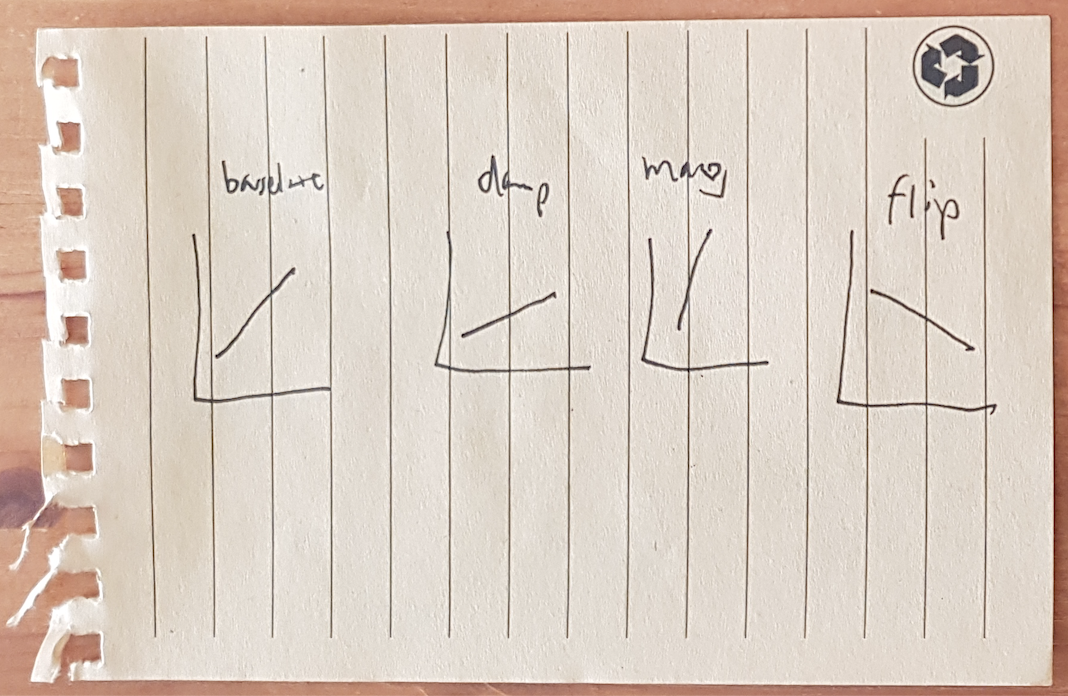
\includegraphics[width=1.0\textwidth,page=1]{mainmatter/figures/chapter_01/fig_mockup_reQTLs_Screenshot 2020-05-21 at 17.08.49.png}
    \caption{eqtl mech models: magnify, dampen, flip}
    \label{fig:intro_reQTLmechs}
\end{figure}

\1 Given the effect of an eQTL can be starkly different between environments, it is critical to use trait-relevant \gls{eQTL} datasets for target gene prioritisation at GWAS loci.
    \2 It has already been shown that use of relevant cell-type specific eQTLs increases coloc rates with GWAS hits \autocite{kim-hellmuth2019CellTypeSpecific} \url{https://www.ncbi.nlm.nih.gov/pmc/articles/PMC4498151/} \url{https://www.biorxiv.org/content/10.1101/2020.01.15.907436v1}
    \2 Conversely, successful colocalisation of GWAS loci with coloc may prioritise not only the target gene, but the specific environments most relevant to a trait.
    % TODO:  coloc then finemap: also can help fine mapping, as large fx = smaller n required = able to do denser genotypeing by e.g. wgs, so smaller credible sets at much lower sample sizes https://www.biorxiv.org/content/10.1101/2020.01.15.907436v1

\subsection{Immune \Glsfmtlongpl{reQTL}}
\label{subsec:intro_reQTL}

\1 A important subclass of context-dependent \gls{eQTL} are \gls{reQTL}, where the interacting environment is experimental stimulation \autocite{vandiedonck2017GeneticAssociationMolecular,huang2019GeneticsGeneExpression}.
    \2 \textit{In vitro}, potential interacting variables such as cell type, and the nature, length, and intensity of stimulation can be precisely controlled.

\1 A seminal early study was conducted by \autocite{barreiro2012DecipheringGeneticArchitecture}, where eQTLs were mapped separately in monocyte-derived dendritic cells before and after 18h infection with \textit{Mycobacterium tuberculosis}.
    \2 reQTLs were detected for 198 genes, 102 specific to the uninfected state, and 96 specific to the infected state. 

    \2 Since then, \textit{in vitro} immune reQTL studies have been conducted for a variety of 
    cell types
        (e.g. primary CD14+ monocytes \autocite{fairfax2014InnateImmuneActivity}) 
    and stimulations 
    (IFN$\gamma$ and LPS \autocite{fairfax2014InnateImmuneActivity}).

    \todo{list a few more types and stims from \autocite{fairfax2014InnateImmuneActivity} until \autocite{alasoo2019GeneticEffectsPromoter}}
    % 	Found reQTLs? So what? Gather take home messages and inspiration for post reQTL analyses
        % •	reQTL effect characteristation
        % o	reQTLs can show reversal of effect between conditions (Fairfax et al. 2014)
        % •	reQTLs vs expression
        % o	enrichment in DE genes vs eQTLs and non eQTLs (Barreiro et al., 2012)
        % o	context-specific eQTL are identified because of both treatment-induced regulatory effects and treatment-inducing gene expression to detectable levels (Fairfax et al. 2014)
        % •	trans effects
        % o	reQTLs develop trans-effects on stimulation (Fairfax et al. 2014)
        % •	reQTLs in pathways
        % o	Fairfax et al. 2014: reQTLs frequently intersected established canonical pathways of monocyte signaling
        % •	reQTLs enrichment in relevant GWAS hits
        % o	Barreiro et al., 2012
        % o	Fairfax et al. 2014
        % •	genomic feature enrichment of reQTLs in certain feature classes
        % o	UTRs (Fu et al., 2012)
        % •	Overlap of reQTL genes with DE genes
        % o	Franco et al. 2014
        % •	Mediation analysis of eQTL -> Ab response (Franco et al. 2014)
        % •	Colocalisation with GWAS (Kim-Hellmuth et al. 2017)
        % •	motifs enriched at reQTL binding sites e.g. STATs, IRFs (Caliskan et al. 2015; Davenport et al. 2018)
        % 	Gather reQTL datasets for coloc
        % •	Fairfax 2014 stim monocytes
        % •	CEDAR range of resting cells
        % •	Schmiedel_2018 stim CD4/8s
        % •	Alasoo 2018 stim macro
        % •	… and whole blood meta control

\1 A complementary approach is \textit{in vivo} \gls{reQTL} mapping
    \2 There are pros to \textit{in vivo} stimulation.
        \3 the innumerable interactions in the immune system that are absent \textit{in vitro}
        \2 ability to use whole organism perturbations more suited for in vivo administration
        \3 ability to get whole organism phenotypes
        \3 ability to get repeated measures: can reason about change in expression over time
    \2 Major disadvantages: 
        \3 the choice of stimulation must be ethical \textit{in vivo}, 
        \3 and many environmental factors (e.g. diet, lifestyle, immune exposures) cannot be controlled, leading to greater experimental noise (?), and more complex interpretations.

    \2 There are few published \textit{in vivo} \gls{reQTL} studies.
        \3 \autocite{franco2013IntegrativeGenomicAnalysis}: seasonal \gls{TIV}, whole blood, antigen processing and intracellular trafficking genes, attempted mediation for Ab titres, but concluded they were underpowered
        % In addition to DIABLO and TRAPPC4 identified above, several genes identified in the epistatic analysis help regulate apoptosis, including FADD,22 ITK23 and REG3A.24
        \3 \autocite{lareau2016InteractionQuantitativeTrait}: fold-change expression after inactivated vaccinia vaccine, focus was on pairwise epistatic interactions, apoptosis pathways
        % \3 TODO: \autocite{zhernakova2017IdentificationContextdependentExpression}
        \3 \autocite{davenport2018DiscoveringVivoCytokineeQTL}: whole blood, IFN status and anti-IL6 drug exposure, reQTL driven by ISRE and IRF4 motifs

\1 <why care about immune reQTLs>
    \2 Exposes differences in regulatory architecture between conditions. 
    \2 Does not automatically reveal the mechanisms behind those differences, but provides a starting point for forming mechanistic hypotheses e.g. context-specific expression

    \2 Nevertheless useful for interpretation of GWAS signals, providing info on likely contexts that mediate the genetic effect

    \2 Immune \textit{in vitro} \gls{reQTL} have been shown to be enriched more so than non-\gls{reQTL} among GWAS loci for immune-related phenotypes such as
    susceptibility to infectious \autocite{barreiro2012DecipheringGeneticArchitecture,manry2017DecipheringGeneticControl}
    and immune-mediated diseases \autocite{manry2017DecipheringGeneticControl,kim-hellmuth2017GeneticRegulatoryEffects}.
        % TODO
        % \3 some enrichments in specifically stimulated states https://www.nature.com/articles/s41588-019-0505-9

        % TODO
    % davenport
    % eQTL interactions with drug interventions or other therapeutically relevant physiologic variables are important to identify as they can point to regulatory mechanisms, such as transcription factors or subclasses of enhancers, acting downstream of the environmental condition of interest and driving groups of eQTL interactions. The IFN status eQTL interactions we identified provide support for this approach.

    \2 Not yet clear whether \textit{in vivo} reQTL have any utility on top of \textit{in vitro} reQTL for interpreting GWAS loci: not that many studies, and complex interpretations.

    \2 Nevertheless, as the number of cell types systems and stimulations both \textit{in vitro} and \textit{in vivo} increases, the number of known reQTLs continues to grow.

\section{Phenotypes of immune response}

\subsection{High-throughput immunology}

\1 Most \gls{reQTL} studies to date have been conducted on immune cells \textit{in vitro}, 
not only due to the abundance of immune cells easily accessible in peripheral blood, amenable to separation (e.g. FACS) and stimulation;
but because the immune system is specialised for responding to environmental perturbations in the form of infections.
    % TODO: janeway ch1 and 2
    \2 The immune system consists of many cell types: lymphoid and myeloid linages
    \todo{specifically introduce cell types mentioned in later chapters}
    \2 two major components, innate and adaptive.
    \2 complex interactions through cell surface receptors and signalling molecules

\1 omics studies of interactions with and between all these layers of the immune system come under the broad umbrella of systems immunology
    \2 Longitudinal designs and high-throughput technologies to quantify the components of the immune system at baseline, and in response to perturbations.
        \3 genomics, epigenomics, transciptomics, proteomics, cell counts
    \2 Whatever the perturbation, just like for most phenotypes, immune response varies between individuals
    \2 Main types of study are descriptive:
        \3 finding correlations between the components of the immune system, and with phenotypic response
    \2 predictive:
        \3 Use assayed information to predict phenotypic response from molecular assays
    \2 causal:
        \3 Mechanisms of response are important to understand e.g. 
            \4 what mechanisms promote effective responses to pathogens and vaccines
            \4 impede dysregulated responses that lead to immune-mediated disease such as IBD.
    \2 Natural genetic variation can be leveraged, representing small scale perturbations that are causally anchored \autocite{tsang2015UtilizingPopulationVariation,villani2018SystemsImmunologyLearning}
    % TODO: Writ large
        \3 Overall estimates of the heritability of many immune parameters, such as cell composition and serum protein levels, lies between 20-40\% \autocite{liston2016ShapingVariationHuman,brodin2017HumanImmuneSystem,patin2018NaturalVariationParameters,liston2018OriginsDiversityHuman}
        \3 Genetic regulation is more important for the innate immune system than the adaptive immune system \autocite{patin2018NaturalVariationParameters}.

% \subsection{Genetic effects on the healthy immune system}
%
% \1 Heritability of immune phenotypes is not only restricted to the expression phenotypes discussed above.
%     \2 Systems studies of interindividual variation in the healthy immune system shows many aspects of the immune system are heritable and complex.
%         \3 <Systems immunology: just getting started \url{https://www.nature.com/articles/ni.3768}>
%     \2 Immune parameters are influenced by age, sex, seasonality, and chronic infection \autocite{brodin2015VariationHumanImmune,liston2016ShapingVariationHuman,brodin2017HumanImmuneSystem,patin2018NaturalVariationParameters,liston2018OriginsDiversityHuman} \url{https://www.nature.com/articles/ncomms8000},
    % TODO: define aspects, parameters
    % TODO: add https://www.nature.com/articles/ni.3371 "The cellular composition of the human immune system is shaped by age and cohabitation"
%     but most individuals have a healthy baseline immune state that is individual-specific,
%     and relatively stable over time \autocite{liston2016ShapingVariationHuman,brodin2017HumanImmuneSystem,lakshmikanth2020HumanImmuneSystem}.
    % TODO: stable, yet varies by age? respecify scale of stability
    % TODO: add https://www.sciencedirect.com/science/article/abs/pii/S0952791520300698 "Understanding immune variation for improved translational medicine"
%     \2 Overall estimates of the heritability of many immune parameters, such as cell composition and serum protein levels, lies between 20-40\% \autocite{liston2016ShapingVariationHuman,brodin2017HumanImmuneSystem,patin2018NaturalVariationParameters,liston2018OriginsDiversityHuman}
%     \2 Genetic regulation is more important for the innate immune system than the adaptive immune system \autocite{patin2018NaturalVariationParameters}.
%
% \1 given genetic control of healthy system, perhaps not surprising that immune response to perturbation traits are also complex
%     \2 also, as discussed in the context section above, context-specific genetic effects may not be apparent in the baseline healthy state, stimulation is required
%     \2 since a central goal of systems immunology is to establish causal relationships between the many components of the immune system
%         \3 Natural genetic variation can be leveraged, representing small scale perturbations that are causally anchored \autocite{tsang2015UtilizingPopulationVariation,villani2018SystemsImmunologyLearning}
%     \2 In this context, immune in vivo reQTL studies can be considered as controllable perturbation studies of the activated immune system
%         \3 Studies of natural infection are complicated by e.g. determining exposure, ethics, dose
%     \2 Simultaneously provides insight in to the biology behind those specific responses
%     \2 Two immune perturbations considered in this thesis are vaccines and biologic drugs.

\subsection{Immune response to vaccination}
% NOTE: technically vaccines are biologics
\todo{this is a general systems vaccinology review. specific flu studies are reviewed in ch2}

\1 One of the earliest applications of systems immunology was to vaccine response, leading to the sub-discipline of systems vaccinology.
    \2 <general summary of biology of vaccine response, specific flu vaccine biology goes in ch2>
        \3 Vaccines stimulate the immune system with pathogen-derived antigens to induce effector responses (primarily antigen-specific antibodies) and immunological memory against the pathogen itself.
        \3 These effector responses are then be rapidly reactivated in cases of future exposure to the pathogen, mediating long-term protection.
        \3 Non-Ab mediated responses [...]
        % \3 <a bit more on innate/adaptive distinction, B/T lineage distinction>
    \2 Vaccination has enormous impact on global health \autocite{greenwood2014ContributionVaccinationGlobal}
    \2 But traditional vaccine dev is empirical (classical "isolate, inactivate, inject" paradigm), often successful vaccine dev does not offer insights into the mechanisms of efficacy 
    \2 The immunological mechanisms that underpin a specific vaccine's success or failure in a given individual are often poorly understood.
    % <For the majority of licensed vaccines, there is a lack of understanding regarding the molecular mechanisms that underpin this variation in host immune response.>
    \2 A vaccine that is highly efficacious in one human population may have significantly lower efficacy in other populations.
    Particularly challenging populations for vaccination include the infants and elderly, pregnant, immuno compromised patients, ethnically-diverse populations, and developing countries.
        \3 e.g. variable vaccine efficacy of rotavirus vaccine
        \3 e.g. variable efficacy of flu vaccine \url{https://www.sciencedirect.com/science/article/pii/S1473309918304900}

% TODO: figure on innate phase then adaptive response to vacc

% TODO: first year report for sysvacc intro
\1 Systems vaccinology is the application of -omics technologies to provide a systems-level characterisation of the human immune system after vaccine-perturbation.
    % \2 These systems vaccinology studies often consider longitudinal measurements of the transcriptomic, cellular, cytokine, and antibody immune responses following vaccination.
    % \2 Measurements are taken at multiple molecular levels (e.g. genome, transcriptome, proteome), and molecular signatures that correlate with and predict vaccine-induced immunity are identified.
    \2 Systems vaccinology has been successfully applied to a variety of licensed vaccines [yellow fever, influenza ...], and also to vaccine candidates against [HIV, malaria ...], resulting in the identification of early transcriptomic signatures that predict vaccine-induced antibody responses.
    \todo{define what a signature is in terms of correlation and prediction}
        \3 <add more references to lists [...] of what vaccines have been studied>
        % TODO use sysvacc\_review\_docx
    \2 Has revealed many influences on vaccine response (age, sex, dose, adjuvants, expression signatures, microbiome, strain etc.)
    \2 So far, studies have been mainly descriptive and predictive.
    \2 Identifying causal relationships can inform more mechanism-based and cost-effective design (rational paradigm), and the move towards personalised vaccinology.
    \2 Studies of impact of host genetics on response are underrepresented \autocite{linnik2016ImpactHostGenetic}

\1 Like for other complex traits, from twin studies it's known that vaccine Ab responses are heritable.
    \2 Moving out of the candidate gene era (e.g. \url{https://www.ncbi.nlm.nih.gov/pmc/articles/PMC3570049/}) into GWAS.
    % TODO: are there mendellian associations?
    \2 Heritability of vaccine response phenotypes \autocite{oconnor2013CharacterizingVaccineResponses}
    \2 Many loci have been implicated by GWAS e.g. HLA \autocite{oconnor2013CharacterizingVaccineResponses,mooney2013SystemsImmunogeneticsVaccines,mentzer2015SearchingHumanGenetic,linnik2016ImpactHostGenetic,scepanovic2018HumanGeneticVariants,dhakal2019HostFactorsImpact}
    \todo{find best GWAS ref, probably mooney2013SystemsImmunogeneticsVaccines, then prune and reassign these citations}
    % \2 Also, phenotypes such as adverse events have been studied e.g. \url{https://pubmed.ncbi.nlm.nih.gov/25344690/}
    \2 Overall, systems vacc studies that include genetics (sometimes dubbed as vaccinogenomics studies) are nowhere near as mature compared to the trait to gene pipeline described in above e.g. applied to complex disease

\subsection{Immune response to anti-TNF biologics}
\todo{cut this section (???)}
<Considering whether I need a section here on anti-TNFs analogous to the above systems vaccinology section. Much anti-TNF response literature is already reviewed in chapter 4 introduction though, so maybe no point duplicating.>
%
%
% TODO: merge this into intro ch4
% \1 <quick anti-tnf summary, specific ADA/IFX biology goes in ch4>
%     \2 biologics are drugs synthesised using a living organism, typically proteins
%     \2 cause immune response due to having immune targets, or immunogenecity because or their large and complex structure vs chem synth small molecule drugs
%     \2 one of the largest classes are anti-TNFs
%     \2 anti-TNFs (or TNF inhibitors), are drugs that suppress the activity of the TNF signalling pathway of the immune system
        % \3 TNF is an inflammatory cytokine ... inflammation is ...
%     \2 they are used to treat immune-mediated inflammatory diseases e.g. rheumatoid arthritis, Crohn's disease, psoriasis and ankylosing spondylitis.
    % Currently, five biologic agents targeting TNF are approved for the treatment of rheumatoid arthritis (RA), inflammatory bowel disease (IBD; for example, Crohn disease and ulcerative colitis), psoriasis, psoriatic arthritis, ankylosing spondylitis, juvenile idiopathic arthritis (JIA) and, most recently, hidradenitis suppurativa4,5 (TABLE 1).
%         \3 indicated for many IMIDs e.g. rheumatoid arthritis, Psoriasis, ankylosing spondylitis. \autocite{lichtenstein2013ComprehensiveReviewAntitumor,kalliolias2016TNFBiologyPathogenic,mulhearn2019UsingImmunophenotypePredict}
%     \2 an enormous amount of money is spent on them: anti-TNF biologics are some of the largest market share pharmaceuticals
%     \2 some proportion of patients fail. given the expenditures, it would be good to predict this
%
% TODO: figure on TNF pathway with drug targets
% TODO: table of biologics with costs
%
% TODO: merge this intro discussion ch4
% \1 <expression signatures of response to anti-TNFs>
%     \2 Systems immunology has also been applied to anti-TNFs
%     \2 have been detected e.g. for RA <"Validation study of existing gene expression signatures for anti-TNF treatment in patients with rheumatoid arthritis" \url{https://pubmed.ncbi.nlm.nih.gov/22457743/}>
    % e.g. https://www.ncbi.nlm.nih.gov/pmc/articles/PMC6614444/
%     \2 most detected in small cohorts, many require validation
%
% TODO: merge this intro discussion ch4
% \1 <genetics of anti-TNF response>
%     \2 pharmacogenomics is the study of the role of genetics in beneficial and adverse effects of drugs and theraputics \url{https://doi.org/10.1016/S0140-6736(19)31276-0}
%     \2 some implementation in clinic already e.g. screening for certain allele-drug combos \url{https://www.nature.com/articles/nature15817} \url{https://academic.oup.com/bmb/article/124/1/65/4430783}
%     \2 GWAS in the pharmacogenomics field \url{https://www.ncbi.nlm.nih.gov/pmc/articles/PMC3003940/} \url{https://www.futuremedicine.com/doi/full/10.2217/pgs-2018-0204}
    % Genome-wide association studies (GWAS) have proven to be a more successful approach for this objective. To date, eight GWAS on anti-TNF response in RA have been performed (22–29), identifying several loci associated at a genome-wide scale. From these, variation at MED15, GFRA1, PDE3A-SLCO1C1, and CD84 has been replicated in, at least, an independent cohort of patients (30).
%     \2 GWAS studies of anti-TNF response in RA \url{https://www.ncbi.nlm.nih.gov/pmc/articles/PMC6614444/}
        % \3 also add Discovery studies from \url{https://www.ebi.ac.uk/gwas/efotraits/EFO_0004653}
    % \2 TODO: \url{https://www.ebi.ac.uk/gwas/search?query=TNF},
    % also google anti tnf immune response gwas
        % e.g.
        % https://www.ncbi.nlm.nih.gov/pmc/articles/PMC6150911/
        % https://journals.plos.org/plosone/article?id=10.1371/journal.pone.0213073
%         \3 a few validation studies attempted e.g. \url{https://www.ncbi.nlm.nih.gov/pmc/articles/PMC5937760/}
%
% \1 a lot of studies also done for CD and IBD (described in ch4)

\section{Thesis overview}

\1 My thesis focuses on two specific instances of in vivo immune response: antibody response to pandemic influenza vaccine in healthy individuals, and clinical response to biologic anti-TNF therapy for CD patients.
\1 <By chapter context-content-conclusion overview.>
    \2 <ch 2: systems vaccinology study of Pandemrix>
        \3 context: existing Sobolev study of expression differences between pandemic flu vaccine R/NR had small sample size and binary phenotype
        \3 content: meta-analysis of existing array with new RNAseq data and continuous phenotype
        \3 conclusion: distinct innate and adaptive expression response at d1 and d7; heterogeneity between array and RNAseq. significant expression differences between R/NR in meta-analysis at the gene set level
    \2 <ch 3: in vivo reQTL study of Pandemrix>
        \3 context: relatively few studies have assessed the impact of genetic variation on expression response to flu vaccine
        \3 content: reQTL analysis for flu vaccine at d0, d1, d7. many reQTLs including sign flips. no particular gene set enrichments. evidence of cell type interactions at top hits.
        \3 conclusion: difficult to separate out modifying effect of cell composition. this may be a fundamental flaw in the study design
    \2 <ch 4: systems immunology and reQTL study of response to anti-TNF treatment in CD>
        \3 context: studies on expression signatures of anti-TNF PNR have been small
        \3 content: R/NR comparison with larger n, at baseline, w14, and over time. reQTL analysis over 4 timepoints. 
        \3 conclusion: a few hits for PNR at baseline. much stronger expression differences stronger at w14, then maintained until w54. Weak evidence for reQTLs, probably due to smaller magnitude of cell proportion changes over time vs the previous chapter.
    \2 <discussion: limitations, future outlook>
        \3 main themes and parallels tying together the thesis
        \3 shared set of limitations permeating all chapters
        \3 recommendations for future analyses and study design
        \3 future outlook for the fields of systems studies of immune response% vaccinogenomics and pharmacogenomics

\end{outline}
